\documentclass[12pt]{article}
\usepackage{amsmath}
\usepackage{amssymb}
\usepackage[letterpaper,top=1.2in,bottom=1in,left=0.75in,right=0.75in,centering]{geometry}
%\usepackage{fancyhdr}
\usepackage{enumerate}
%\usepackage{lastpage}
\usepackage{multicol}
\usepackage{graphicx}

\reversemarginpar

%\pagestyle{fancy}
%\cfoot{}
%\lhead{Math 1560}\chead{Test \# 1}\rhead{May 18th, 2017}
%\rfoot{Total: 10 points}
%\chead{{\bf Name:}}
\newcommand{\points}[1]{\marginpar{\hspace{24pt}[#1]}}
\newcommand{\skipline}{\vspace{12pt}}
%\renewcommand{\headrulewidth}{0in}
\headheight 30pt

\newcommand{\di}{\displaystyle}
\newcommand{\abs}[1]{\lvert #1\rvert}
\newcommand{\len}[1]{\lVert #1\rVert}
\renewcommand{\i}{\mathbf{i}}
\renewcommand{\j}{\mathbf{j}}
\renewcommand{\k}{\mathbf{k}}
\newcommand{\R}{\mathbb{R}}
\newcommand{\aaa}{\mathbf{a}}
\newcommand{\bbb}{\mathbf{b}}
\newcommand{\ccc}{\mathbf{c}}
\newcommand{\dotp}{\boldsymbol{\cdot}}
\newcommand{\bbm}{\begin{bmatrix}}
\newcommand{\ebm}{\end{bmatrix}}                   
                  
\begin{document}


\author{Instructor: Sean Fitzpatrick}
\thispagestyle{empty}
\vglue1cm
\begin{center}
{\bf MATH 2565 - Tutorial \#7 Solutions}
\end{center}
\textbf{Assigned problems:}

 \begin{enumerate}
\item Evaluate the indefinite integral:
\begin{enumerate}

 \item $\di \int e^{\sqrt{x}}\,dx$ (Hint: try a substitution first.)

First let $x=u^2$, so $dx=2u\,du$, giving us
\begin{align*}
 \int e^{\sqrt{x}}\,dx &= \int 2ue^u\,du = 2\int u d(e^u) = 2ue^2-2\int e^u\,du = 2ue^u-2e^u+C\\
& = 2\sqrt{x}e^{\sqrt{x}}-2e^{\sqrt{x}}+C.
\end{align*}

 \item $\di \int \cos(x)\cos(2x)\,dx = \int \cos(x)(1-2\sin^2x)\,dx = \sin(x)-\frac{2}{3}\sin^3(x)+C.$

Alternatively, one could use the identity
\[
\cos(ax)\cos(bx)=\frac12\left(\cos(ax+bx)+\cos(ax-bx)\right)
\]
to write $\cos(x)\cos(2x) = \frac12 \cos(3x) + \frac12 \cos(x)$, giving
\[
\int \cos(x)\cos(2x)\,dx = \frac12 \int(\cos(3x)+\cos(x))\,dx = \frac16\sin(3x)+\frac12\sin(x)+C.
\]

 \item $\di \int \frac{\sqrt{5-x^2}}{x^2}\,dx$

\medskip

Letting $x=\sqrt{5}\sin\theta$, so $\sqrt{5-x^2} = \sqrt{5}\cos\theta$ and $dx = \sqrt{5}\cos\theta\,d\theta$, we have
\begin{align*}
 \int\frac{\sqrt{5-x^2}}{x^2}\,dx &= \int \frac{5\cos^2\theta}{5\sin^2\theta}\,d\theta = \int\cot^2\theta\,d\theta = \int (\csc^2\theta-1)\,d\theta\\
 & = -\cot\theta-\theta+C = -\frac{\sqrt{5-x^2}}{x}-\sin^{-1}\left(\frac{x}{\sqrt{5}}\right)+c
\end{align*}


 \item $\di \int \frac{16x^2-2x}{(x+3)(2x-1)(x-1)}\,dx$

We look for a partial fraction decomposition 
\[
\dfrac{16x^2-2x}{(x+3)(2x-1)(x-1)} = \dfrac{A}{x+3}+\dfrac{B}{2x-1}+\dfrac{C}{x-1}. 
\]


Multiplying both sides of this decomposition by $x+3$ gives us 
\[
 \dfrac{16x^2-2x}{(2x-1)(x-1)} = A +\dfrac{B(x+3)}{2x-1}+\dfrac{C(x+3)}{x-1}.
\]
 Plugging in $x=-3$ then gives
$A=\dfrac{75}{14}$.

Multiplying both sides of the decomposition by $2x-1$ gives 
\[
 \dfrac{16x^2-2x}{(x+3)(x-1)} = \dfrac{A(2x-1)}{x+3}+B+\dfrac{C(2x-1)}{x-1},
\]
 and plugging in $x=1/2$ gives $B = \dfrac{12}{7}$.

Multiplying both sides of the decomposition by $x-1$ gives 
\[
 \dfrac{16x^2-2x}{(x+3)(2x-1)} = \dfrac{A(x-1)}{x+3}+\dfrac{B(x-1)}{2x-1}+C,
\]
 and plugging in $x=1$ gives $C=\dfrac{7}{2}$.

Putting everything together, we get
\begin{align*}
 \int \frac{16x^2-2x}{(x+3)(2x-1)(x-1)}\,dx &= \frac{75}{14}\int\frac{1}{x+3}\,dx +\frac{12}{7}\int\frac{1}{2x-1}\,dx + \frac{7}{2}\int\frac{1}{x-1}\,dx\\
& = \frac{75}{14}\ln\abs{x+3}+\frac{6}{7}\ln\abs{2x-1}+\frac{7}{2}\ln\abs{x-1}+C.
\end{align*}

\end{enumerate}



  \item Evaluate the improper integral, or explain why it does not exist:
\begin{enumerate}
 \item $\di \int_0^\infty e^{4-3x}\,dx\lim_{t\to \infty}\int_0^t e^{4-3x}\,dx = \lim_{t\to\infty}\frac{1}{3}(e^4-e^{4-3t})=e^4.$
 

 
 \item $\di \int_{-\infty}^\infty \frac{1}{4+x^2}\,dx = \lim_{s\to\infty}\int_{-s}^0\frac{1}{4+x^2}\,dx+\lim_{t\to\infty}\int_0^t\frac{1}{4+x^2}\,dx$.

Now we recall that $\di \int \frac{1}{4+x^2}\,dx = \frac{1}{2}\tan^{-1}(x/2)$, $\tan^{-1}(0)=0$, and $\lim_{x\to\pm\infty}\tan^{-1}x = \pm \frac{\pi}{2}$. It follows that $\lim_{x\to\infty}\tan^{-1}(\pm x/2) = \pm \frac{\pi}{2}$, since $x/2\to \infty$ if $x\to \infty$. Thus, we get
\[
 \int_{-\infty}^\infty \frac{1}{4+x^2}\,dx = -\frac{1}{2}\lim_{s\to \infty}\tan^{-1}(-s/2)+\frac{1}{2}\lim_{t\to\infty}\tan^{-1}(t/2) = \frac{\pi}{2}.
\]
\end{enumerate}

\newpage

 \item Find the area between the  curves
$y=\sqrt{x}$, $y=-2x+3$, and $y=-\frac{1}{2}x$.


\begin{multicols}{2}
We begin by sketching the region.

We can see from the sketch that it's necessary to break up the area into two regions.
\begin{center}
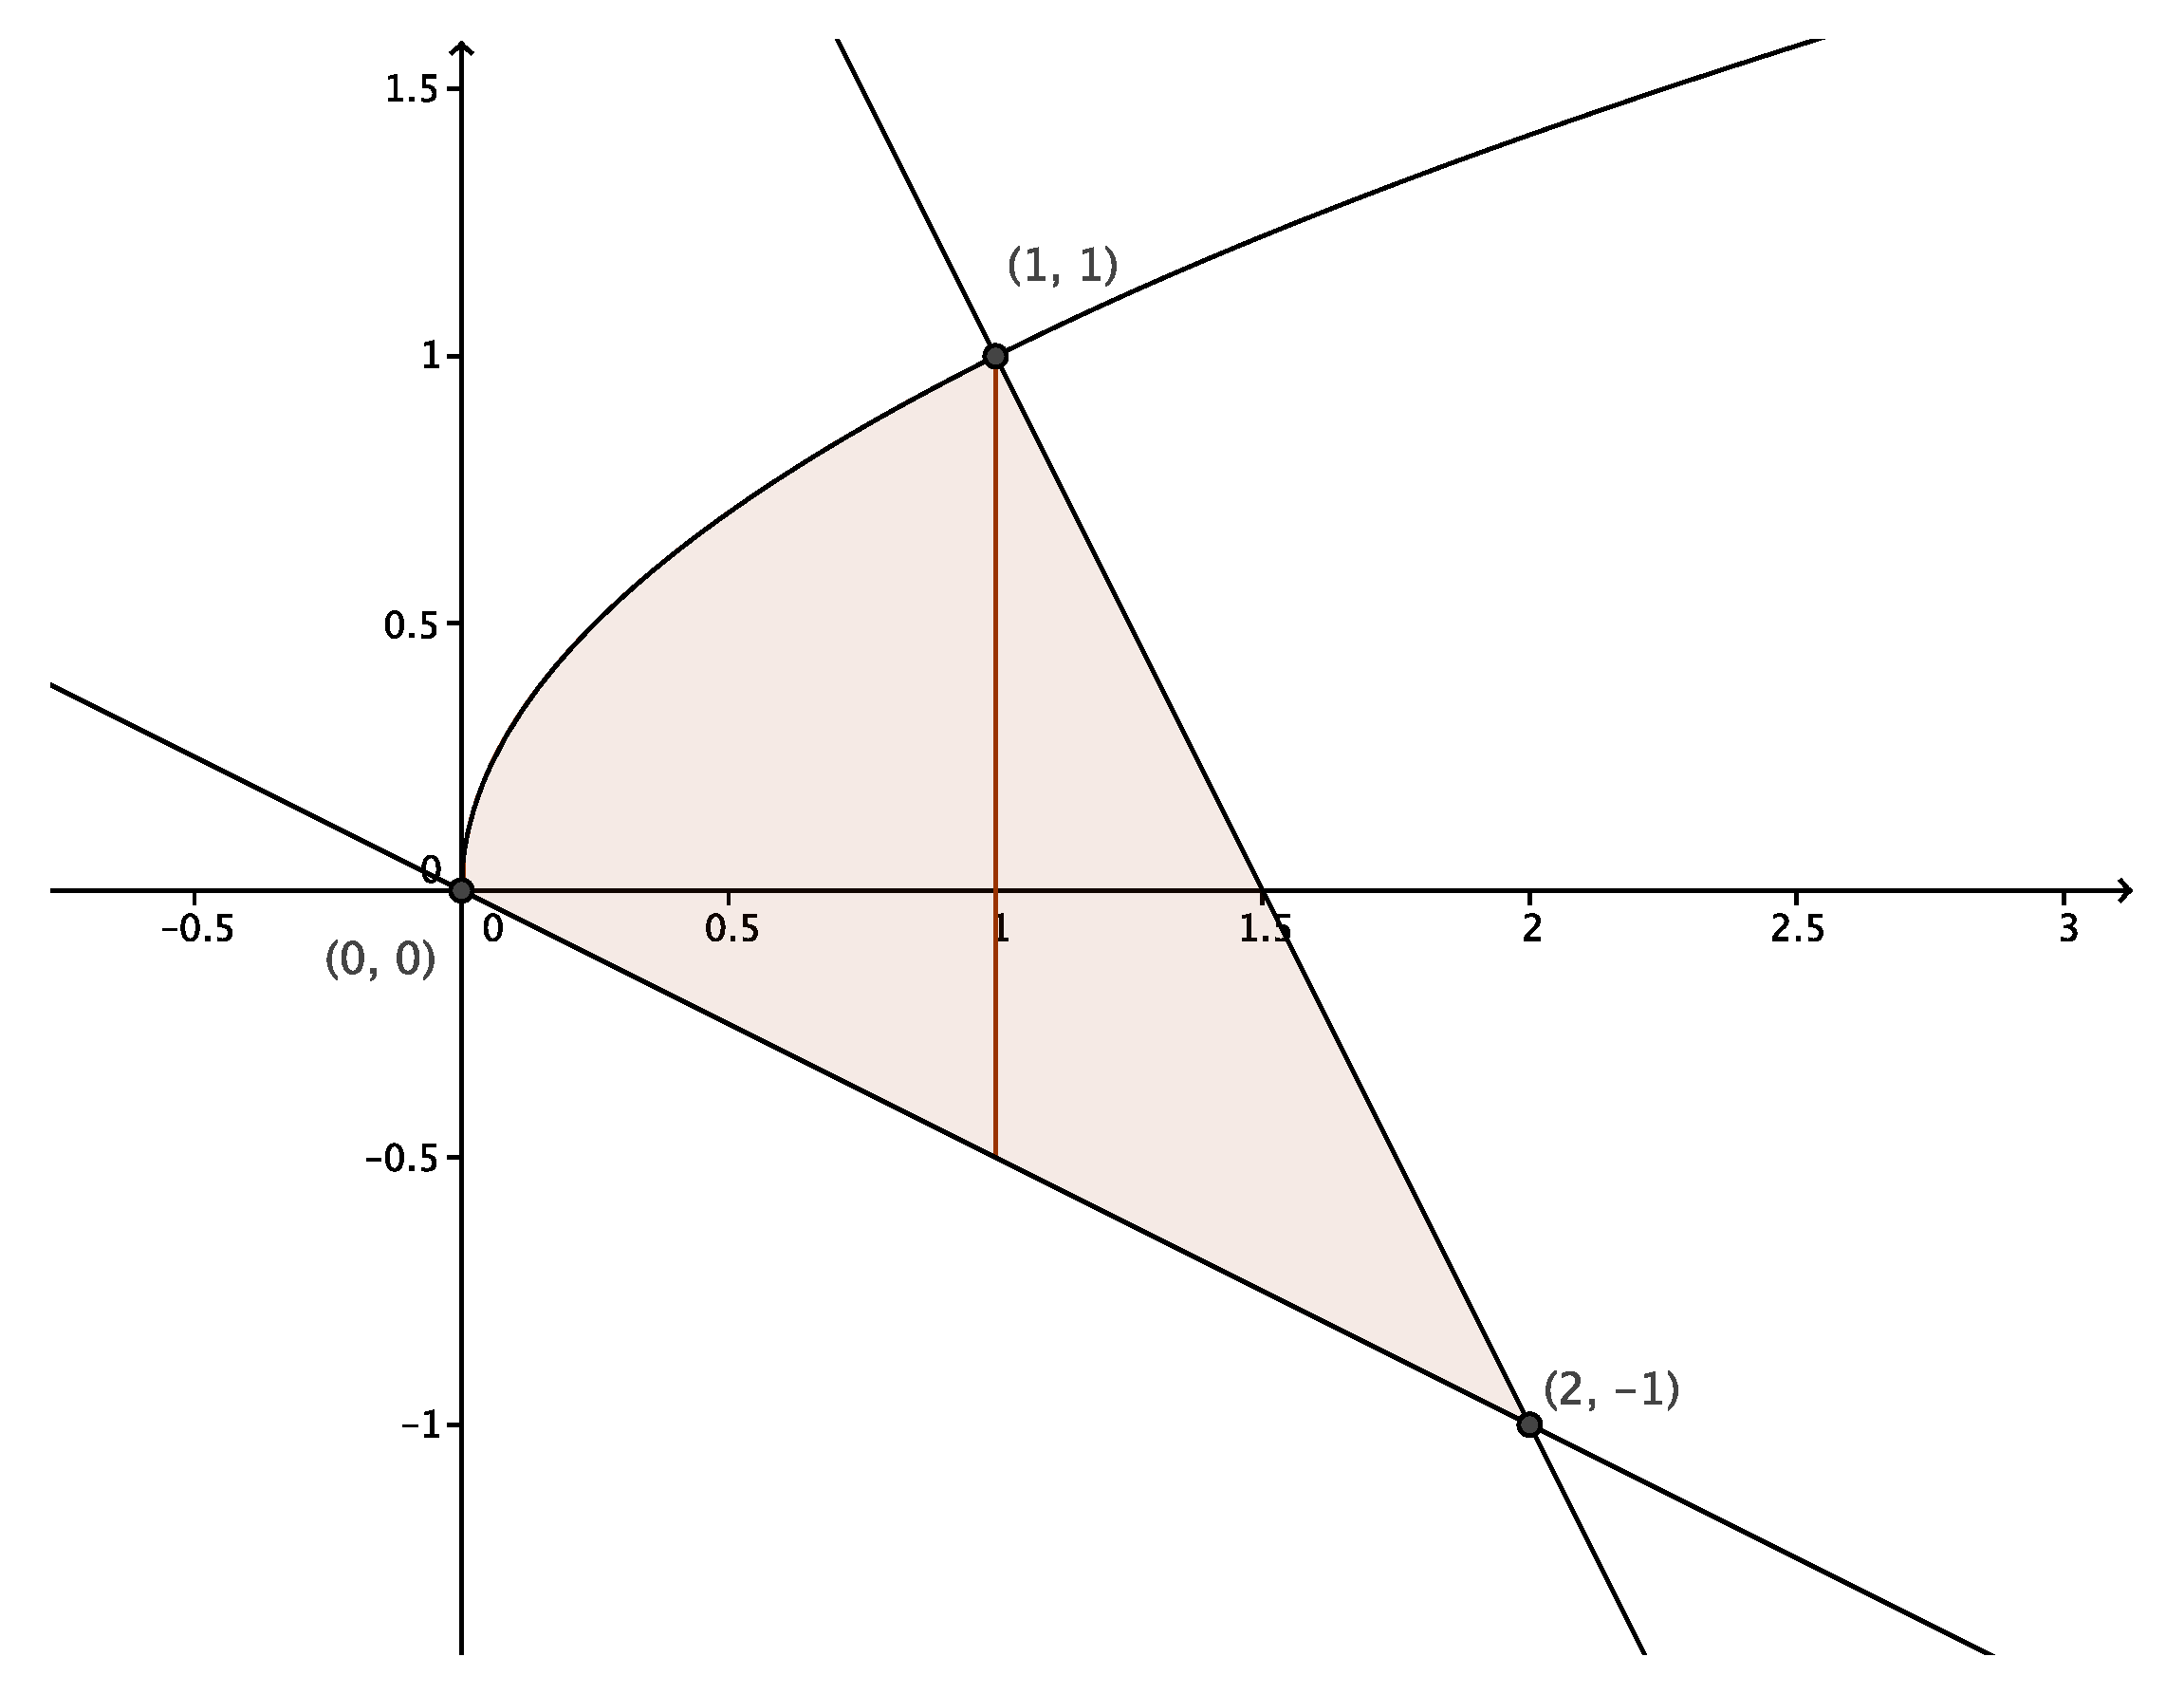
\includegraphics[width=0.4\textwidth]{WS7-2b}
\end{center}
\end{multicols}
 For $0\leq x\leq 1$, the upper curve is $y=\sqrt{x}$ and the lower curve is $y=-\frac{1}{2}x$, giving us the area
\[
 A_1 = \int_0^1\left(\sqrt{x}+\frac{1}{2}x\right)\,dx =\frac{11}{12}.
\]
For $1\leq x\leq 2$, the upper curve changes to $y=3-2x$, giving the area
\[
 A_2 = \int_1^2\left(3-2x+\frac{1}{2}x\right)\,dx = \frac{3}{4}.
\]
The total area is therefore $A=A_1+A_2 = \frac{5}{3}$.

\item Find the volume of the solid of revolution:
\begin{enumerate}
 
 \item Generated by revolving the region bounded by $y=x^2-2x+2$ and $y=2x-1$ about the line $y=1$.

\bigskip

We first sketch the region:
\begin{multicols}{2}
\begin{center}
 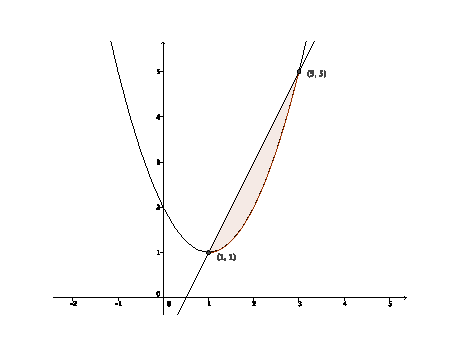
\includegraphics[width=\columnwidth]{WS7-3a}
\end{center}

Since the axis of rotation is vertical this time, we want to use shells in order to integrate with respect to $x$. The radius of each shell is $r(x)=x-1$, and the height is given by the difference in the $y$-values of the two curves: $h(x)=(2x-1)-(x^2-2x+2) = -x^2+4x-3$.
\end{multicols}
Thus, we have
\[
 V = 2\pi\int_1^3 (x-1)(-x^2+4x-3)\,dx = \frac{8\pi}{3}.
\]

 \item Generated by revolving the triangle with vertices $(1,1), (1,2)$, and $(2,1)$ about the $x$-axis.
 \begin{multicols}{2}
 In the additional practice, we found that the volume obtained by revolving this region about the $x$-axis was $4\pi/3$. The symmetry of the region suggests that we should get the same answer when revolving about the $y$-axis. Let's confirm.
 \begin{center}
 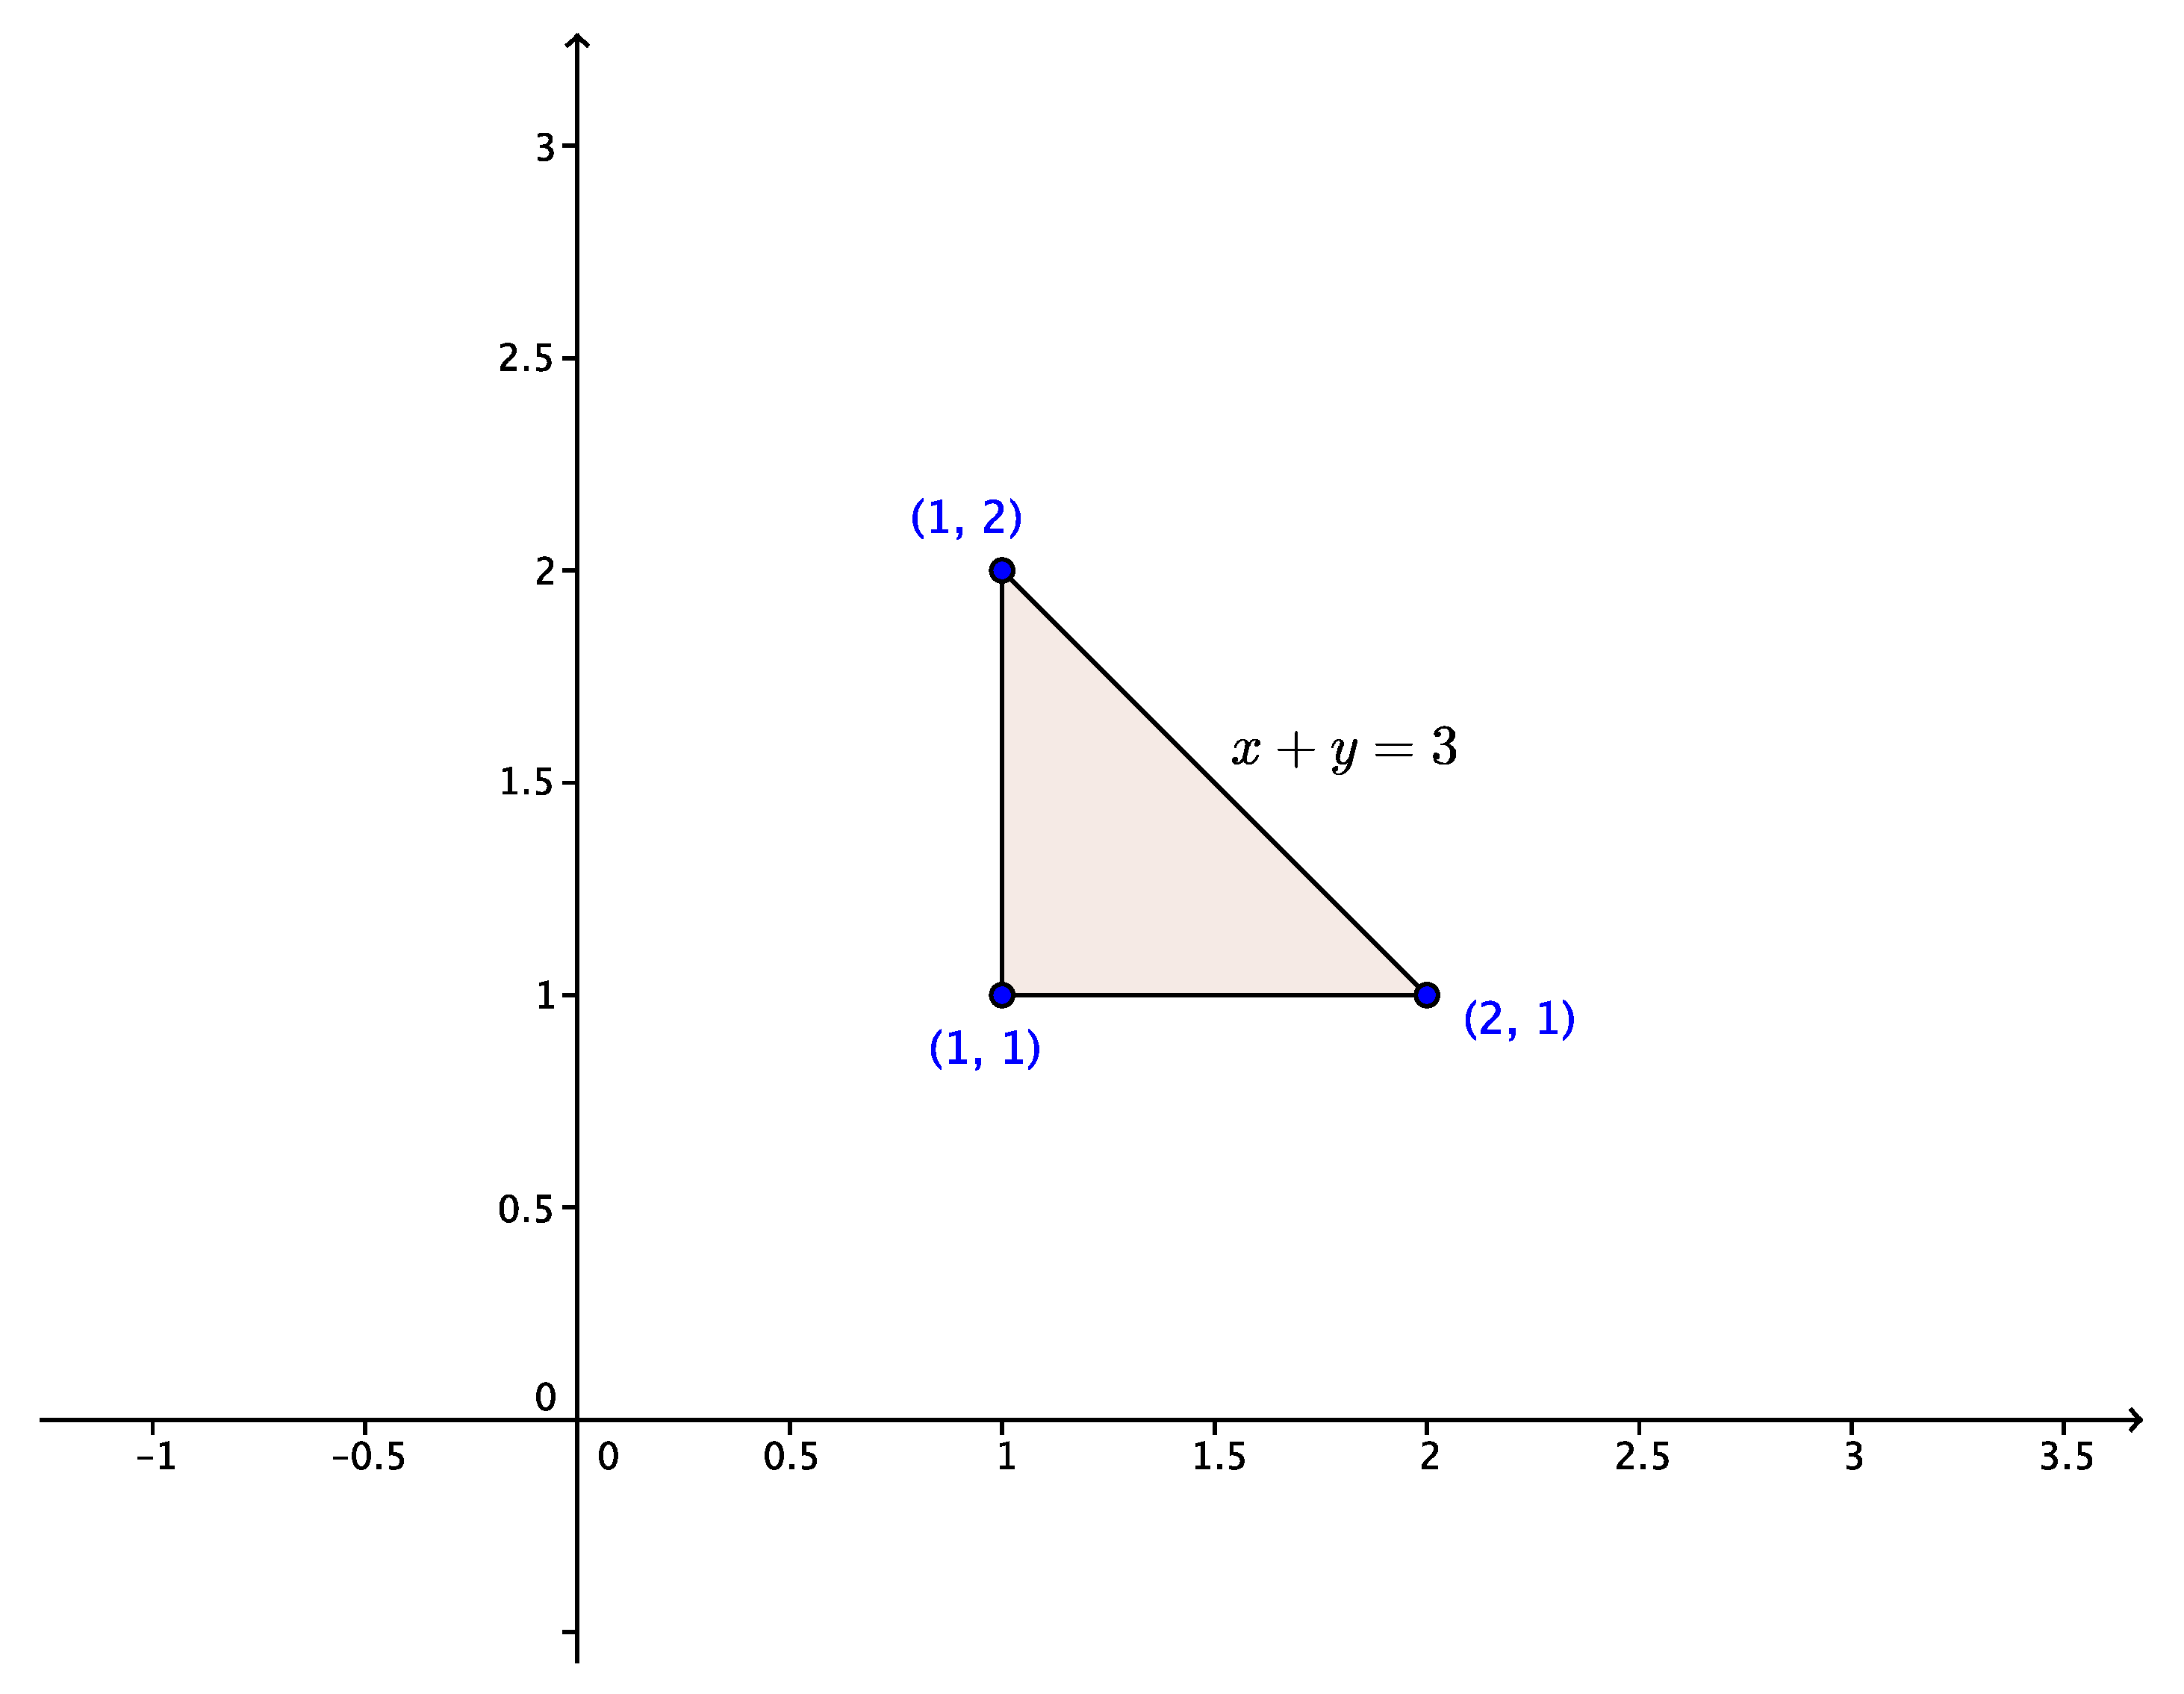
\includegraphics[width=0.8\columnwidth]{WS7-3c}
\end{center}
\end{multicols}


Since the axis is vertical, if we use shells, the integral is with respect to $x$, with $r=x$ and $h=(3-x)-1=2-x$, for $1\leq x\leq 2$. This gives 
\[
V = 2\pi\int_1^2 x(2-x)\,dx = 2\pi\left.\left(x^2-\frac13 x^3\right)\right|_1^2 = 2\pi\left(\left(4-\frac83\right)-\left(1-\frac13\right)\right)=\frac{4\pi}{3},
\]
as expected. If you used washers instead, the integral is with respect to $y$, with $r_{\text{in}}=1$ and $r_{\text{out}}=3-y$, so again we get
\[
V = \pi\int_1^2(3-y)^2-1^2)\,dy = \pi\left.\left(-\frac13 (3-y)^3-y\right)\right|_1^2 = \pi\left(\left(-\frac13-2\right)-\left(-\frac83-1\right)\right)=\frac{4\pi}{3}.
\]
\end{enumerate}




\item Find the area of the surface generated by revolving the the curve $y=x^2$, for $0\leq x\leq 1$, about the $y$-axis.

\bigskip

Since we're revolving about the $y$-axis, we use the formula $S = 2\pi\int_a^b x\sqrt{1+(y')^2}\,dy$, giving us
\[
 S = 2\pi\int_0^1 x\sqrt{1+(2x)^2}\,dx = \frac{\pi}{6}(5\sqrt{5}-1).
\]
 
\end{enumerate}
\newpage

\textbf{Additional practice} (don't include your solutions here):
\begin{enumerate}
\item Evaluate the indefinite integral:

\begin{enumerate}
 \item $\di \int x\sec^2(x)\,dx = \int x d(\tan x) = x\tan x-\int \tan x\,dx = x\tan x+\ln\abs{\cos(x)}+C$
 \item $\di \int \tan^5(x)\sec^4(x)\,dx = \int \tan^5(x)(1+\tan^2(x))\sec^2(x)\,dx = \frac{1}{6}\tan^6(x)+\frac{1}{8}\tan^8(x)+C$
 \item $\di \int \frac{8}{\sqrt{x^2+2}}\,dx$
 
 \medskip

Letting $x=\sqrt{2}\tan\theta$, we have $\sqrt{x^2+2} = \sqrt{2\sec^2\theta} = \sqrt{2}\sec\theta$ and $dx = \sqrt{2}\sec^2\theta\,d\theta$, so
\[
 \int\frac{8}{\sqrt{x^2+2}}\,dx = \int \frac{8\sqrt{2}\sec^2\theta}{\sqrt{2}\sec\theta}\,d\theta = 8\ln\abs{\sec\theta+\tan\theta}+C = 8\ln\abs{x+\sqrt{x^2+2}}+C.
\]
 \item $\di \int \frac{2x+1}{x^3+x}\,dx$
 
 This time we look for a decomposition $\dfrac{2x+1}{x(x^2+1)} = \dfrac{A}{x}+\dfrac{Bx+C}{x^2+1}$. Getting a common denominator on the right-hand side, we have
\[
 \frac{2x+1}{x^3+x} = \frac{Ax^2+A+Bx^2+Cx}{x^3+x}.
\]
Comparing numerators, we have $0x^2+2x+1 = (A+B)x^2+Cx+A$. Constant terms must be equal, so $A=1$, Coefficients of $x$ must be equal, so $C=2$. Coefficients of $x^2$ must be equal, so $A+B=0$, giving $B=-A=-1$. Thus,
\[
 \int\frac{2x+1}{x^3+x}\,dx = \int \frac{1}{x}\,dx -\int\frac{x}{x^2+1}\,dx + 2\int \frac{1}{x^2+1}\,dx = \ln\abs{x}-\frac{1}{2}\ln(x^2+1)+2\tan^{-1}(x)+C.
\]
\end{enumerate}

\item Evaluate the improper integral, or explain why it doesn't exist:

\begin{enumerate}
 \item $\di \int_{-\infty}^\infty \frac{x}{1+x^2}\,dx = \int_{-\infty}^0 \frac{x}{1+x^2}\,dx + \int_0^\infty\frac{x}{1+x^2}\,dx$.

This integral diverges, since both of the two integrals on the right-hand side above diverge. Note that $\di \int\frac{1}{1+x^2}\,dx = \frac{1}{2}\ln(1+x^2)$, and as $x\to \pm\infty$, $\ln(1+x^2)\to\infty$.


 \item $\di \int_1^\infty\frac{\ln x}{x^2}\,dx$
 
 \medskip
 
 Using integration by parts, $\di\int\frac{\ln x}{x^2}\,dx = -\frac{\ln x}{x}-\frac{1}{x}$. We thus have
\begin{align*}
 \int_1^\infty\frac{\ln x}{x^2}\,dx & = \lim_{t\to\infty}\int_1^t \frac{\ln x}{x^2}\,dx\\
& = \lim_{t\to\infty}\left(1-\frac{1}{t}-\frac{\ln t}{t}\right) = 1,
\end{align*}
where we have used the limits $\di\lim_{t\to\infty}\frac{1}{t} = 0$ and (using L'Hospital's rule for the indeterminate form $\infty/\infty$)
\[
 \lim_{t\to\infty}\frac{\ln t}{t} = \lim_{t\to\infty}\frac{1/t}{1} = 0.
\]
\end{enumerate}

\item Find the volume of the solid of revolution:
\begin{enumerate}
\item Generated by revolving the region bounded by $y=x^2-2x+2$ and $y=2x-1$ about the $x$-axis.

\begin{center}
 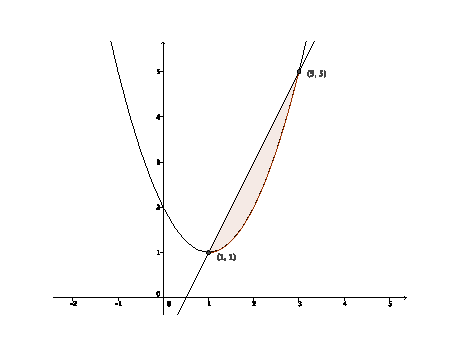
\includegraphics[width=0.5\textwidth]{WS7-3a}
\end{center}

The region for parts (a) and (b) is shown above. Since we're revolving about the $x$-axis for part (a), the washer method is more convenient, as it involves an integral with respect to $x$. (The shell method would require us to solve for $x$ as a function of $y$.)

The outer radius for our washer is given by the value of the $y$-coordinate of the curve that is furthest from the $x$-axis, so we have $r_{out} = 2x-1$. The inner radius is given by the closer of the two curves, so $r_{in} = x^2-2x+2$. Putting these into the formula for volume by washers gives us
\begin{align*}
 V & = \pi\int_1^3 \left[(2x-1)^2-(x^2-2x+2)^2\right]\,dx\\
& = \pi\int_1^3 (-x^4+4x^3-4x^2+4x-3)\,dx = \frac{104\pi}{15}.
\end{align*}
(I don't promise that I avoided computational errors on this one!)

 \item Generated by revolving the triangle with vertices $(1,1), (1,2)$, and $(2,1)$ about the $y$-axis.
 
 \begin{center}
 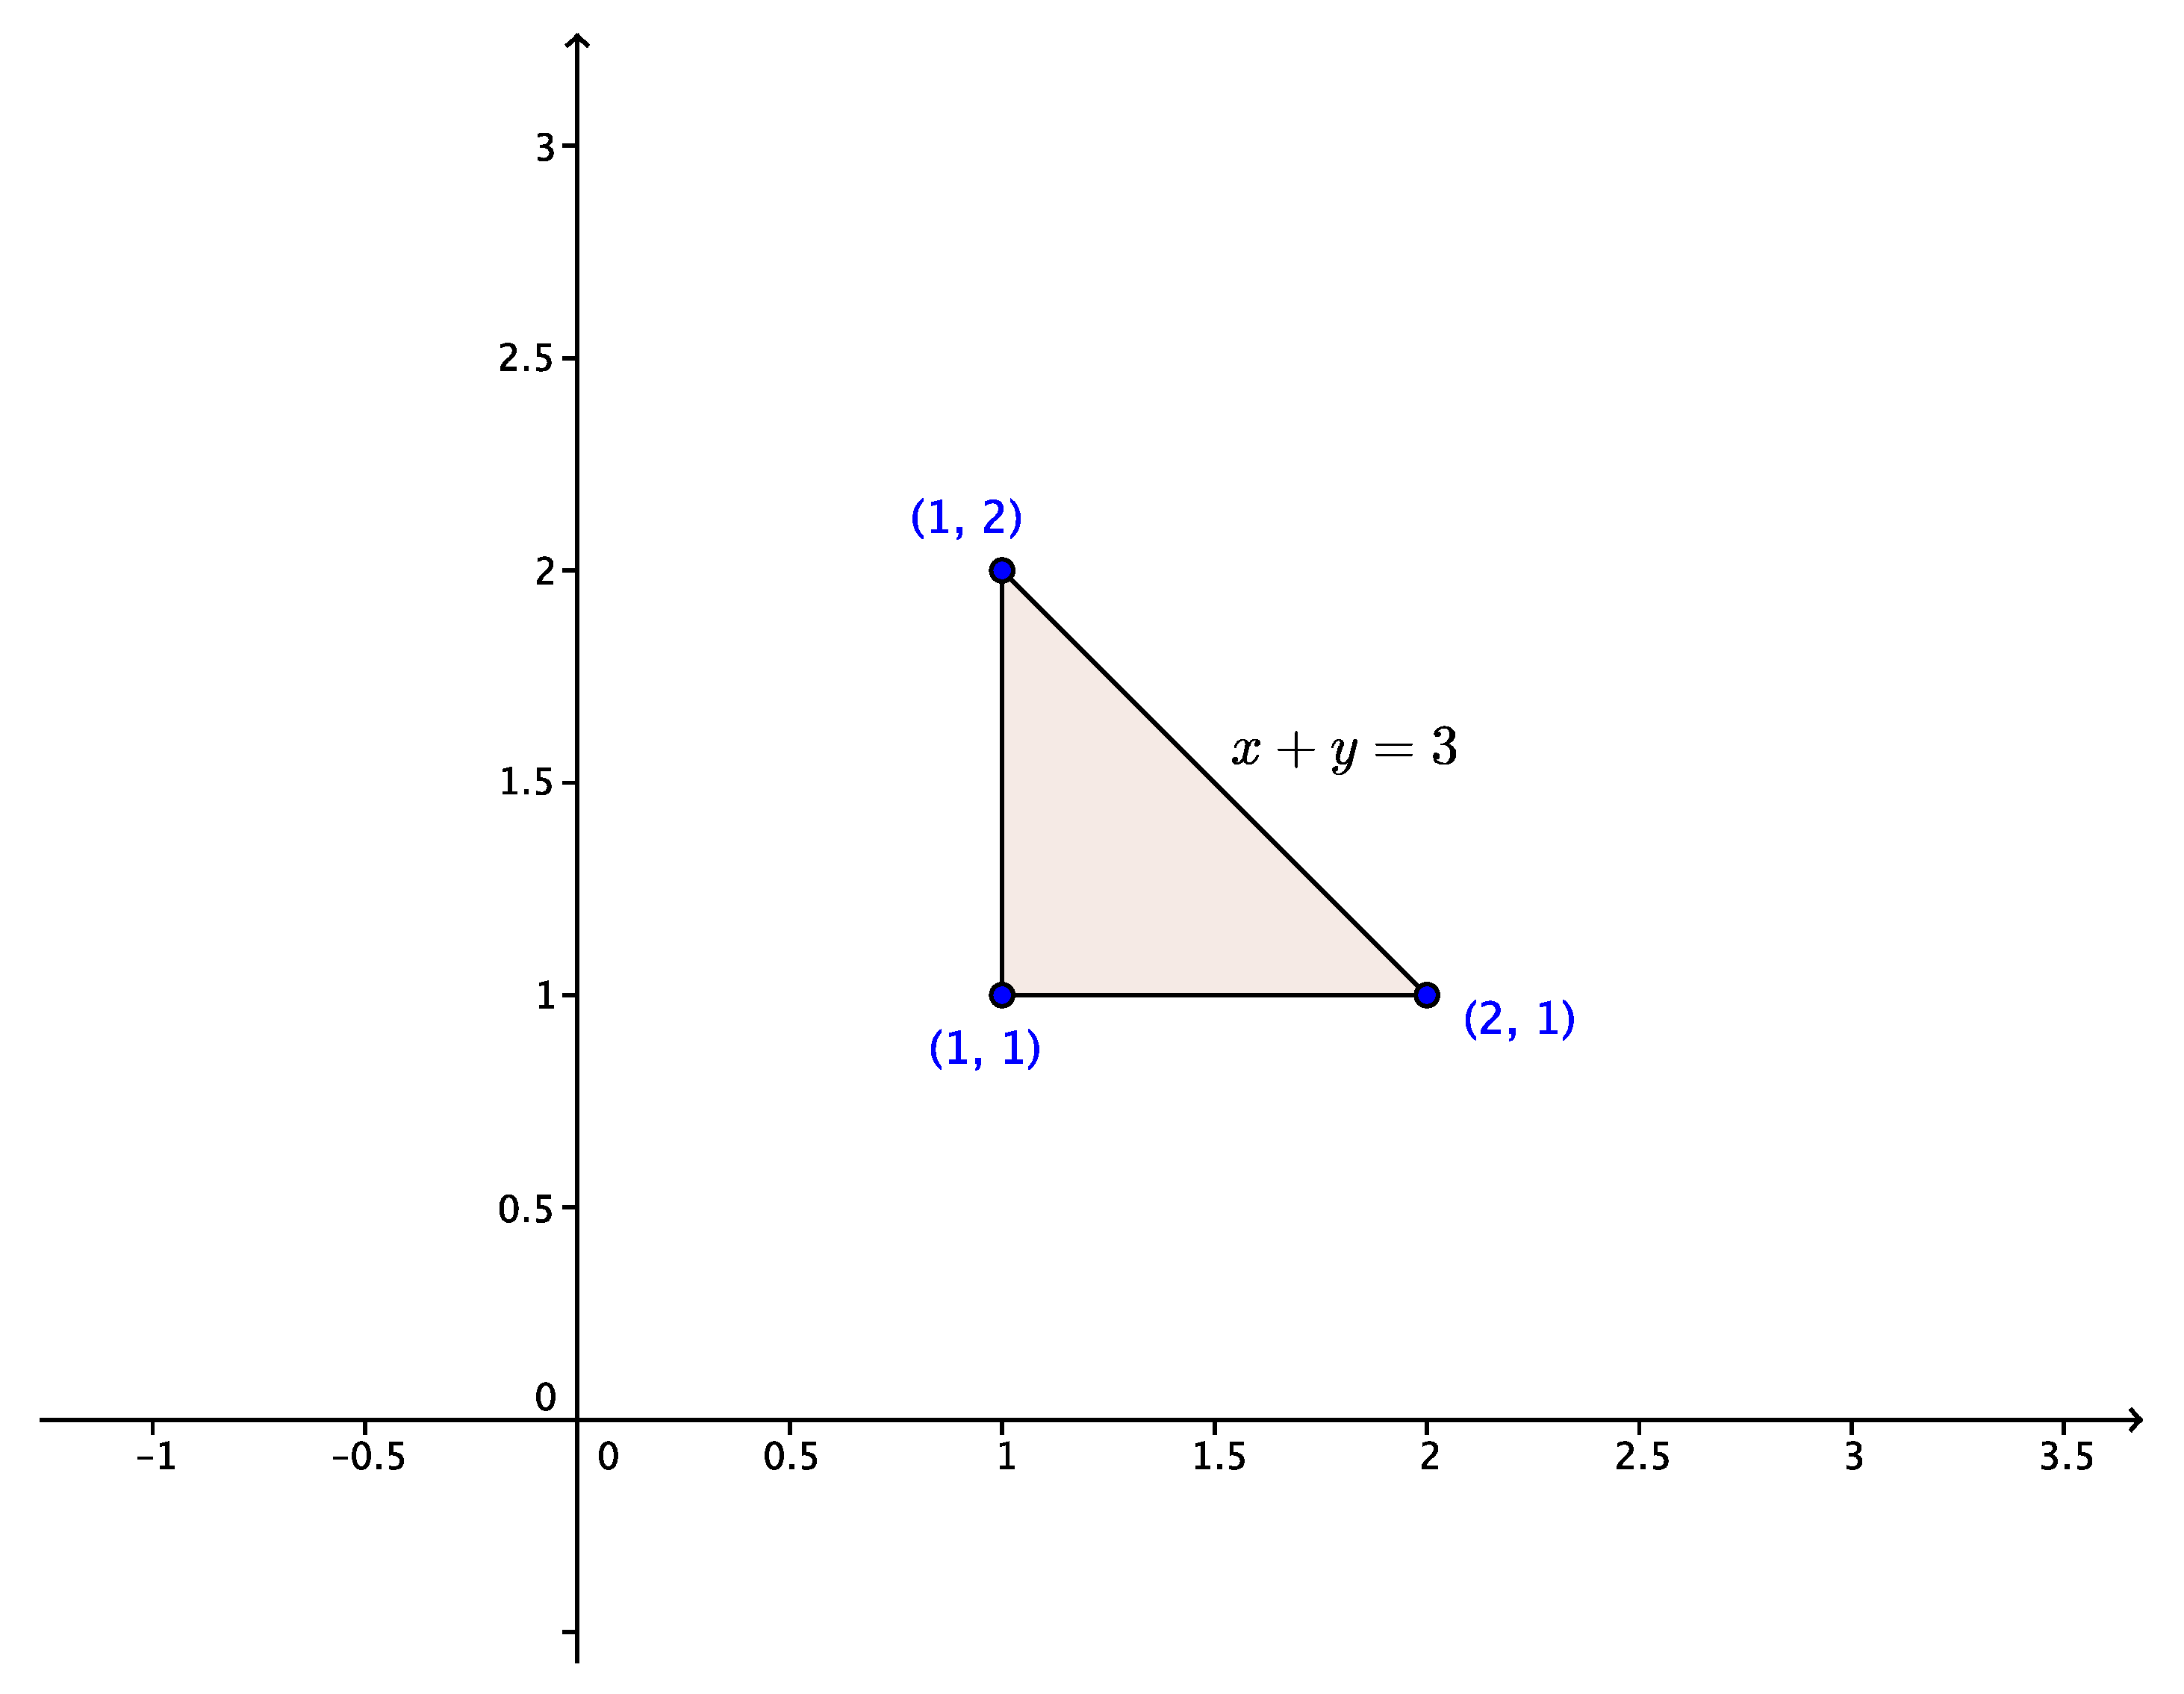
\includegraphics[width=0.5\textwidth]{WS7-3c}
\end{center}

The region to be revolved is shown above. If we choose to use washers, then we write the equation of the hypotenuse of the triangle as $x=3-y$, since we integrate with respect to $y$ for a vertical axis. The inner radius is simply 1 (the vertical side of the triangle), so we have (as seen in tutorial)
\[
 V = \pi\int_1^2[(3-y)^2-1]\,dy = \frac{4\pi}{3}.
\]
If we choose to use shells instead, then the radius of the shell is $x$, and the height is $(3-x)-1 = 2-x$, giving us
\[
 V = 2\pi\int_1^2 x(2-x)\,dx = \frac{4\pi}{3}.
\]

\end{enumerate}
\item Find the length of the curve $y=2x^{3/2}-\dfrac{1}{6}\sqrt{x}$, for $0\leq x\leq 9$.

Since $y' = 3\sqrt{x}-1/(12\sqrt{x})$, we have
\[
 1+(y')^2 = 1+\left(3\sqrt{x}-\frac{1}{12\sqrt{x}}\right)^2 = 1+9x-\frac12 +\frac{1}{144x} = 9x + \frac12 + \frac{1}{144x} = \left(3\sqrt{x}+\frac{1}{12\sqrt{x}}\right)^2.
\]
Thus, the length is
\[
 L = \int_0^9\sqrt{1+(y')^2}\,dx = \int_0^9 \left(3x^{1/2}+\frac{1}{12}x^{-1/2}\right)\,dx = \frac{107}{2}.
\]
\end{enumerate}


%\thispagestyle{empty}






\end{document}